\section{Le langage GRAFCET}

Le langage GRAFCET, aussi appelé SFC (Sequentiel Function Chart) est, comme son nom l'indique, dédié à la description et à la programmation de \textbf{problèmes séquentiels}. Il décrit donc une suite d'étapes séparées par des transitions.

Un GRAFCET est très proche conceptuellement d'une machine à état. Il est représenté tel que sur la Figure~\ref{fig:simpleGrafcet}

\begin{figure}[ht]
  \centering
  \begin{tikzpicture}
\EtapeInit[0,0]{100}
\Transition[VX100]{100}
\Etape[VT100]{110}
\Transition{110}
\Etape[VT110]{120}
\Transition[VX120]{120}
\LienRetour{T120}{X100}
\Recept{T100}{$dcy \cdot a_0$}
\ActionX{X110}{Sortir Noyau}
\Recept{T110}{condition}\ActionX{X120}{Rentrer Noyau}
\Recept{T120}{$a_0$}
\end{tikzpicture}

  \caption{GRAFCET simple composé de trois étapes}
  \label{fig:simpleGrafcet}
\end{figure}

\subsection{Étapes et actions}

Une étape est représentée par un carré comportant un numéro (Figure~\ref{fig:etape}). Elle est généralement associée à une  (Figure~\ref{fig:etapeAction}) ou plusieurs (Figure~\ref{fig:etapeDeuxActions}) actions.
Il est également possible d'ajouter une condition à une action (Figure~\ref{fig:etapeActionCond}).

\UPSTIaRetenir{\begin{itemize}
  \item Une action associée à une étape n'est effectuée que lorsque l'action associée est active.
  \item Une action conditionnelle est effectuée lorsque l'action est active et que la condition associée est vérifiée.
\end{itemize}}

Il également possible d'effectuer une action qu'au moment de l'activation d'une étape (Figure~\ref{fig:etapeActivation}). Cela est particulièrement utile pour incrémenter un compteur.
En effet, sans cela l'action \textit{compteur = compteur + 1} serait effectuée durant toute la durée de l'action associée. Cela incrémenterait le compteur à chaque cycle automate donc toutes les \SI{10}{ms} approximativement.

On peut représenter l'étape actuellement active dans un grafcet à l'aide d'une étoile comme illustré sur la Figure~\ref{fig:etapeActive}.

\begin{figure}[ht]
\centering
  \begin{subfigure}[b]{.49\textwidth}
    \centering
    \begin{tikzpicture}
      \Etape[0,0]{110}
    \end{tikzpicture}
    \caption{Représentation d'une étape en GRAFCET}
    \label{fig:etape}
  \end{subfigure}%
  %
  \begin{subfigure}[b]{.49\textwidth}
    \centering
  \begin{tikzpicture}
    \Etape[0,0]{110}
    \ActionX{X110}{Sortir Noyau}
  \end{tikzpicture}
  \caption{Une étape et l'action associée}
  \label{fig:etapeAction}
  \end{subfigure}%
  %

  \begin{subfigure}[b]{.48\textwidth}
    \centering
  \begin{tikzpicture}
    \Etape[0,0]{110}
    \ActionX{X110}{Sortir Noyau, Allumer voyant}
  \end{tikzpicture}
  \caption{Une étape et deux actions simultanées. Les deux actions sont actives tant que l'étape 110 est active.}
  \label{fig:etapeDeuxActions}
  \end{subfigure}\hfill
%
  \begin{subfigure}[b]{.48\textwidth}
    \centering
  \begin{tikzpicture}
    \Etape[0,0]{110}
    \ActionX{X110}{Sortir Noyau}
    \ActionCond{X110}{$\overline{\text{defaut}}$}
  \end{tikzpicture}
  \caption{Une étape avec action conditionnelle : L'action \textit{Sortir Noyau} ne sera exécutée que si \textit{defaut} est à 0.}
  \label{fig:etapeActionCond}
  \end{subfigure}%

  \begin{subfigure}[b]{.48\textwidth}
    \centering
  \begin{tikzpicture}
    \Etape[0,0]{130}
    \ActionX{X130}{compteur = compteur + 1;}
    \ActionActiv{X130}
  \end{tikzpicture}
  \caption{Une étape et une action sur activation. L'action n'est effectuée qu'au moment de l'activation de l'étape.}
  \label{fig:etapeActivation}
  \end{subfigure}%
  %
  \begin{subfigure}[b]{.48\textwidth}
    \centering
  \begin{tikzpicture}
    \Etape[0,0]{110}
    \ActionX{X110}{Sortir Noyau}
    %\ActionCond{X110}{$\overline{\text{defaut}}$}
    \LienActivation{X110}
  \end{tikzpicture}
  \caption{Etape courramment active}
  \label{fig:etapeActive}
  \end{subfigure}
  \caption{Etapes et action(s) associée(s)}%
  %
\end{figure}


\subsection{Transitions}

Une transition est \textbf{toujours} placée entre deux actions. Ce sont les transitions qui décrivent la façon de passer d'une action à une autre.
Une transition est associée à une \textbf{réceptivité} (Voir Figure~\ref{fig:transition}).

\UPSTIaRetenir{Une transition sera franchie si et seulement si l'étape précédente est active ET la réceptivité associée est vérifiée.}

\begin{figure}[ht]
  \centering
  \begin{subfigure}[b]{.48\textwidth}
    \centering
      \begin{tikzpicture}
        \Transition[0,0]{110}
      \end{tikzpicture}
    \caption{Une transition}
    \label{fig:transition}
  \end{subfigure}
  \begin{subfigure}[b]{.48\textwidth}
    \centering
      \begin{tikzpicture}
        \Transition[0,0]{110}
        \Recept{T110}{$dcy \cdot a_0$}
      \end{tikzpicture}
    \caption{Une transition et sa réceptivité associée}
    \label{fig:transitionEtRecept}
  \end{subfigure}
  \caption{Transitions et Réceptivité}
  \label{fig:transition}
\end{figure}

\subsection{Saut d'étapes et reprise de séquence}
Le saut d'étapes permet de sauter une ou plusieurs étapes lorsque les actions associées sont inutiles à réaliser, La reprise de séquence (ou boucle) permet de reprendre, une ou plusieurs fois, une séquence tant qu'une condition n'est pas obtenue.


\subsection{Divergences et Convergences}
\subsubsection{Divergence/Convergence en OU}
On dit qu'il y a Aiguillage ou divergence en OU lorsque le grafcet se décompose en deux ou plusieurs séquences selon un choix conditionnel. Comme la divergence en OU on rencontre aussi la convergence en OU. On dit qu'il y a convergence en OU, lorsque deux ou plusieurs séquences du grafcet converge vers une seule séquence.

 Un exemple est donnée en Figure~\ref{fig:divOU}.

\UPSTIaRetenir{\begin{itemize}
  \item Une convergence en \textbf{OU} commence \textbf{toujours} par une transition sur chacune de ses branches.
  \item Une convergence en \textbf{OU} se termine \textbf{toujours} par une transition sur chacune de ses branches.
  \item Les conditions d'une divergence doivent être exclusives.
\end{itemize}}

\begin{figure}[ht]
  \centering
  \begin{tikzpicture}
  \Etape[0,0]{1}
  \DivOU{X1}{-5/L1a,3/L1b,11/L1c}
  \SequenceTT[L1a]{1a}{11}
  \SequenceTT[L1b]{1b}{21,22,23}
  \SequenceTT[L1c]{1c}{31,32}
  \ConvOU[-3]{T23}{T32,T11}{L2}
  \Etape[L2]{2}
  \DecaleNoeudy[-3]{VX2}{VX2}
  \DecaleNoeudy[-3]{NoeudGraf}{NoeudGraf}
  \Actions{1/A1,11/A11,21/A11,22/A22,
  23/A23,31/A31,2/A2}
  \Recepts{1a/r1a,1b/r1b,1c/r1c,11/r11,
  21/r21,22/r22,23/r23,31/r31,32/r32}
\end{tikzpicture}

  \caption{Exemple de divergence en \textbf{OU}. Une seule des branches est parcourrue.}
  \label{fig:divOU}
\end{figure}


\subsubsection{Divergence en ET}
Au contraire de l'aiguillage où ne peut se dérouler qu'une seule activité à la fois, On dit qu'on se trouve en présence d'un parallélisme structurel, si plusieurs activités indépendantes pouvant se dérouler en parallèle. Le début d'une divergence en ET et la fin d'une convergence en ET d'un parallélisme structurel sont représentés par deux traits parallèles. Un exemple est donnée en Figure~\ref{fig:divET}.

\UPSTIremarque{La dernière étape d'une divergence en ET est souvent vide pour attendre les autres branches.}
\begin{figure}
  \centering
  \begin{tikzpicture}
  \Etape{3}
  \Transition{3}
  \DivET{T3}{-6/br1,7/br3,20/br2}
  \Graphe[Vbr1]{
  21/Remplir cuve/ cuver remplie
  }
  \Etape{24}
  \Etape[Vbr2]{31}
  \SequenceEE[Vbr3]{11,12}{13}
  \ConvET[-7]{X13}{X24,X31}{b40}
  \Transition[b40]{40}
  \Etape{41}
  \ActionRecept{
  11/Sortir tige verin/tige sortie,
  12/Rentrer tige verin/tige rentrée
  }
  \ActionX{X31}{Allumer voyant}
  \Recept{T3}{$marche$}
  \Recept{T40}{$\underline1$}
\end{tikzpicture}

  \caption{Exemple de divergence en \textbf{ET}. Les trois branches sont parcourrue simultanéement.}
  \label{fig:divET}
\end{figure}

\subsection{Rêgles de conception}
\UPSTIaRetenir{\begin{itemize}
  \item Les actions ne concernent que les \textbf{actionneurs} ou des variables internes.
  \item Les réceptivités ne concernent que les capteurs ou des variables internes
  \item Une étape est \textbf{toujours} suivie d'une transition
  \item Une transition est \textbf{toujours} suivie d'une étape.
\end{itemize}}
